% ex: ts=2 sw=2 sts=2 et filetype=tex
% SPDX-License-Identifier: CC-BY-SA-4.0
\begin{frame}
    \frametitle{Contenido}
    \tableofcontents
\end{frame}

\section{Definiciones básicas}

\begin{frame}[c]{Conceptos}
  \begin{itemize}
    \item Un algoritmo se pude escribir en diferentes idiomas o
      \textbf{lenguajes}.
    \pausa
    \item Un \textbf{programa} es un algoritmo escrito en \textbf{lenguaje
      máquina}.
    \pausa
    \item El \textbf{programador} se encarga de desarrollar los programas
      computacionales.
    \pausa
    \item Los programadores utilizan:
      \begin{itemize}
        \item Lenguajes de programación
        \pausa
        \item Compiladores
        \pausa
        \item Interpretes
        \pausa
        \item Enlazadores
        \pausa
        \item Depuradores (debuggers)
        \pausa
        \item Entornos de desarrollo integrados (IDEs)
      \end{itemize}
      para realizar sus programas.
  \end{itemize}
\end{frame}

\begin{frame}[c]{Conceptos}
  \begin{itemize}
    \item Para poder desarrollar un programa es necesario utilizar un
      \textbf{lenguaje de programación}.
    \pausa
    \item Cada lenguaje de programación define reglas de escritura:
      \textbf{Léxicas}, \textbf{sintácticas} y \textbf{semánticas}.
    \pausa
    \item Existen muchos lenguajes de programación:
      \begin{multicols}{3}
        \begin{itemize}
          \item C
          \pausa
          \item C++
          \pausa
          \item C\#
          \pausa
          \item Java
          \pausa
          \item JavaScript
          \pausa
          \item Python
          \pausa
          \item PHP
          \pausa
          \item Go
          \pausa
          \item Rust
        \end{itemize}
      \end{multicols}
  \end{itemize}
\end{frame}

\begin{frame}[c]{Conceptos}
  \begin{itemize}
    \item Las instrucciones que escribió el programador forman el
      \textbf{código fuente} (source code). Entonces, el código fuente es un
      algoritmo escrito utilizando un lenguaje de programación.
    \pausa
    \item Un \textbf{compilador} es un programa que se encarga de traducir
      el código fuente a un código objeto (obj), y que junto un enlazador
      (linker) genera un programa en lenguaje máquina directamente ejecutable.
    \pausa
    \item El \textbf{lenguaje máquina} es aquél que es entendido y ejecutado
      por una computadora. En Windows tienen la extinción \textbf{exe} y
      \textbf{dll}.
  \end{itemize}
\end{frame}

\begin{frame}[c]{Conceptos}
  \begin{itemize}
    \item Un \textbf{intérprete} es un programa que se encarga de traducir
      línea a línea el código fuente y ejecutar las acciones. \emph{No genera
      un ejecutable}.
      \begin{itemize}
        \item Hay lenguajes interpretados, como \textbf{Python}, que no usan
          compilador, sino un intérprete; el intérprete es diferente al
          compilador, porque genera el código máquina sin generar un archivo
          ejecutable (\textbf{exe} o \textbf{dll}, por ejemplo).
      \end{itemize}
    \pausa
    \item Un \textbf{enlazador} es un programa que toma el código objeto
      generado por un proceso de compilación y enlaza dicho código con sus
      bibliotecas para generar un archivo ejecutable.
  \end{itemize}
\end{frame}

\begin{frame}[c]{Conceptos}
  \begin{itemize}
    \item Un \textbf{depurador} (debugger en ingles) se encarga de probar y
      eliminar errores. Incorpora funcionalidades como ejecutar un programa
      paso a paso, pausar el programa, dar seguimiento a los valores de
      algunas variables.
    \pausa
    \item Un \textbf{entorno de desarrollo integrado} (IDE) agrupa servicios y
      herramientas para facilitarle el desarrollo de software a los
      programadores.
  \end{itemize}
\end{frame}

\section{Fases de un programa}

\begin{frame}[c]{Código fuente, Objeto y ejecutable}
  \begin{center}
    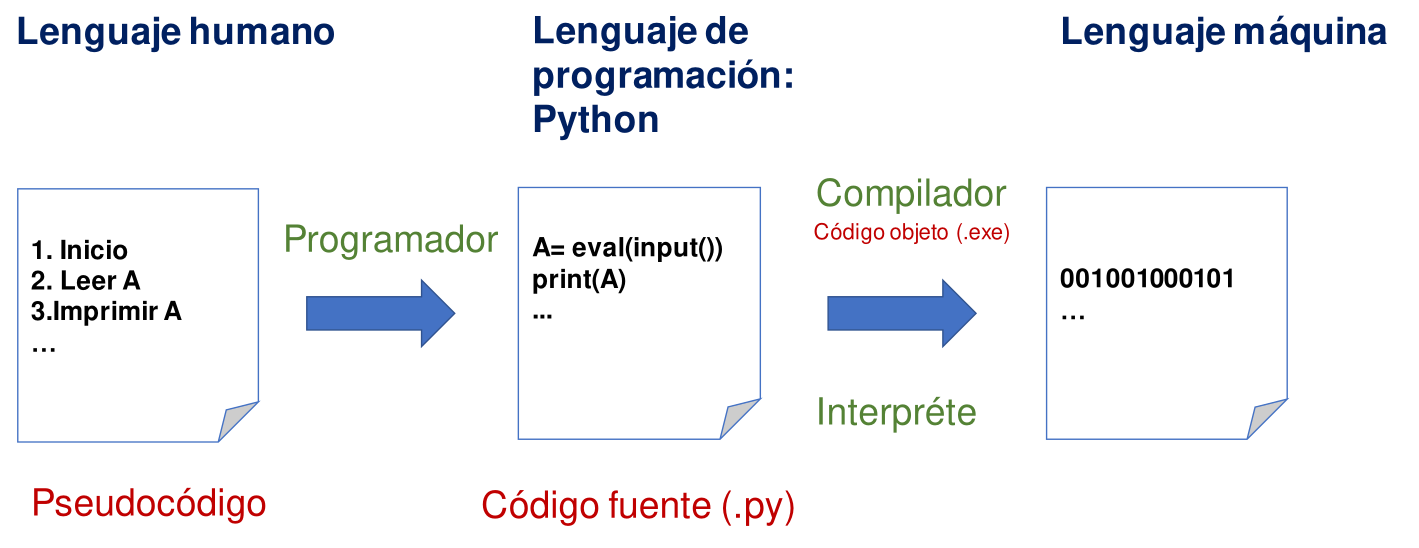
\includegraphics[scale=0.3]{011_fuente_objeto_ejecutable.png}
  \end{center}
\end{frame}

\begin{frame}[c]{Intérprete, compilador y enlazador}
  Proceso que sigue cada uno de los traductores para la ejecución de un
  programa:
  \begin{center}
    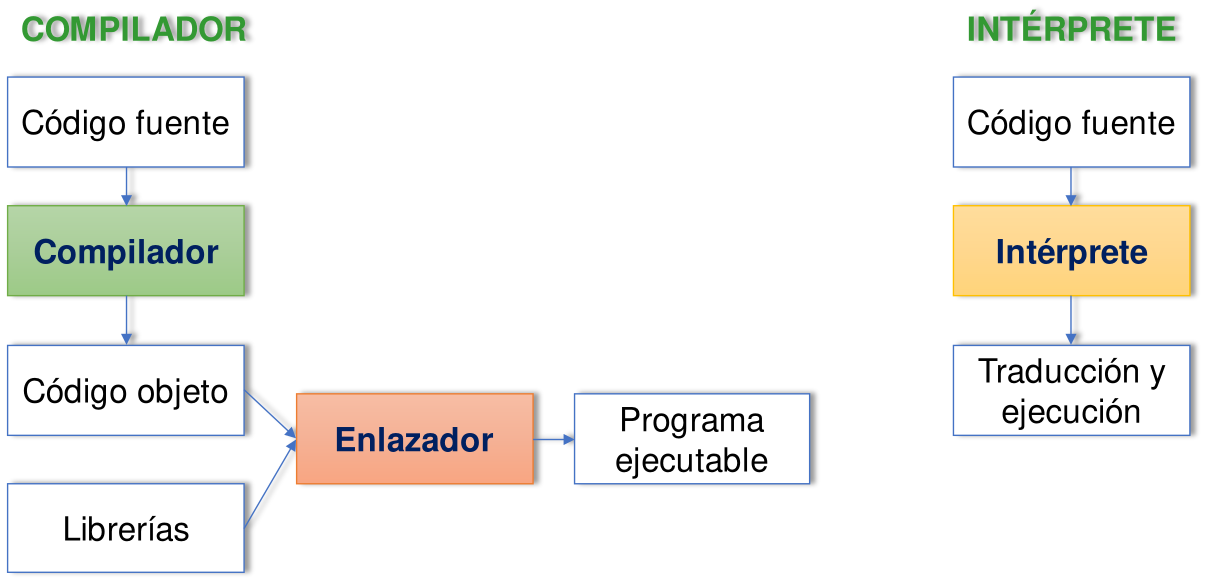
\includegraphics[scale=0.28]{011_compilador_interprete.png}
  \end{center}
\end{frame}

\section{Entornos de desarrollo integrados}

\begin{frame}[c]{Conceptos}
  \begin{itemize}
    \item Es un entorno de programación que al menos incluye un editor de
      código, un compilador o intérprete, un depurador y un constructor de
      interfaz gráfica (GUI).
    \pausa
    \item Una herramienta que provee un marco de trabajo amigable
    \pausa
    \item Generalmente tiene las siguientes características:
      \begin{itemize}
        \item Multiplataforma
        \pausa
        \item Soporte para diversos lenguajes de programación
        \pausa
        \item Integración con Sistemas de Control de Versiones
        \pausa
        \item Reconocimiento de Sintaxis
        \pausa
        \item Depurador
        \pausa
        \item Múltiples idiomas
        \pausa
        \item Manual de Usuarios y Ayuda
      \end{itemize}
  \end{itemize}
\end{frame}
